\subsection{Fonctionnement et développement de la plante}

\subsubsection{Généralités}

Tout d'abord, présentons succintement comment se développe et fonctionne une plante. 
La science qui décrit l'ensemble des mécanismes qui participent à l'édification d'un organsime vivant est appelée morphogénèse

Chez les plantes, la morphogénèse commence avec la germination de la graine et s'arrète à la mort de la plante.~\cite[p.~22]{these_modelisation}.
Celle-ci diffère d'une plante à l'autre, et dépend également de l'environnement de la plante.

Ce sont les méristèmes\footnote{Le méristème est un tissu formé de cellules indiffériencées (embryonnaires) qui se divisent activement et permettent la croissance.} qui permettent à la plante de se développer, en allongeant des organes déjà existants ou en créant de nouveaux organes.
Lors de la germination de la graine, au stade embryonnaire, des méristèmes permettent déjà le développement de la plante (méristèmes racinaires, caulinaires).
On distingue les méristèmes végétatifs, à l’origine des organes végétatifs (tige, feuilles, racines) et les méristèmes reproducteurs, à l’origine des fleurs.
On distingue également les méristèmes primaires, qui permettent à la plante de croître en longueur (tiges et racines) et les méristèmes secondaires, qui permettent la croissance en épaisseur de la plante.
La création de nouveaux organes est réalisée par alignement de nouvelles briques élémentaires (formée par les méristèmes), constituées :
\begin{itemize}
	\item d'un noeud, auquel sont liés les feuilles
	\item d'un entrenoeud 
	\item d'un bourgeon situé à la base du noeud, à l'aisselle des feuilles
\end{itemize} 

Ces briques élémentaires sont appelées phytomères. Cette caractéristique permet de simplifier la modélisation de la croissance d'une plante.



\subsubsection{Photosynthèse}
\label{subsubsec:photosynthese}
Sans doute que la particularité la plus intéressante des plantes, et qui justifie le mieux leur étude est leur capacité à synthétiser de la matière organique (des glucides...) à partir de \ce{CO2}, d'eau et d'énergie solaire. C'est la célèbre photosynthèse qui permet ainsi à la plante de 
transformer de la matière \emph{minérale} en matière \emph{organique},
selon l'équation
\begin{equation}
	\ce{6CO2 + 6H2O + \text{énergie solaire} -> C6H12O6 + O2 }.
  \label{eq:photosynthese}
\end{equation}

Tous les éléments de la plante participent à ce processus de photosynthèse :
\begin{itemize}
	\item les racines puisent dans le sol l'eau et les sels minéraux nécessaires		
	\item les feuilles captent l'énergie solaire et le dioxyde de carbone 
  (grâce aux cellules chlorophiliennes 
  et aux stomates\footnote{Orifice de petite taille situé sur les feuilles 
  qui permet les échanges gazeux entre l'air et la plante.})
\end{itemize}

\begin{figure}[h]
	\begin{center}
  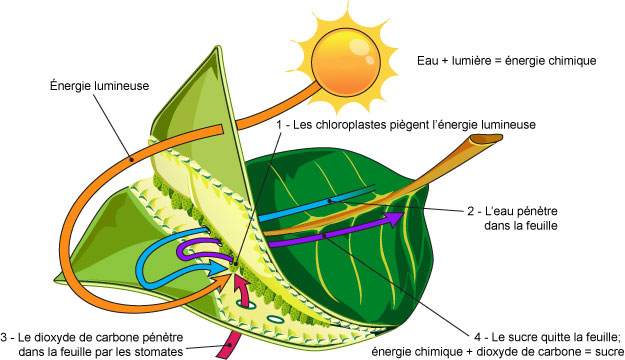
\includegraphics[scale=0.51]{./img/photosynthese.jpg}
  \caption{Photosynthèse}
  \label{fig:photosynthèse}
	\end{center}
\end{figure}

Les sucres ainsi formés apportent l'énergie nécessaire au fonctionnement de la plante et assurent son développement en permettant la synthèse de cellulose qui est l'élément consitutif principal des plantes.
On identifie ainsi les éléments qui agissent sur la croissance de la plante : 
\begin{itemize}
	\item la lumière
	\item l'eau
	\item le dioxyde de carbone
	\item la température : car la température agit sur l'ouverture des stomates et donc sur le flux des échanges gazeux
	\item l'azote, qui permet à la plante de construire les acides aminés nécessaires à l'élaboration des protéines
	\item d'autres minéraux, comme le potassium qui favorise les transferts au sein de la plante
\end{itemize}

Tous les organes de la plante s'unissent donc pour aboutir à la production de biomasse. Cette biomasse est ensuite distribuée aux organes pour permettre leur développement.

Parce que ce mécanisme permet de synthétiser de la matière minérale en matière organique et de capter du \ce{CO2}, gaz à effet de serre notoire, il est crucial de comprendre ce mécanisme de photosynthèse. C'est pourquoi il est, au même titre que la croissance des plantes l'objet de nombreuses recherches (avec comme application : créer de l'électricité propre en dissociant \ce{H2O} en Oxygène et en Hydrogène, capter du \ce{CO2}...

